\chapter{归纳不变式自动生成工具的实现}\label{chap:implementation}

本章节基于设计方案,详细介绍了归纳不变式自动生成工具的实现细节,包括块之间的交互,以及模块的具体实现。

\section{候选不变式检验模块}

候选不变式检验模块主要负责对生成的候选不变式进行验证,检验其正确性,独立性和与已有不变式析取结果的递归性。

候选不变式检验模块接入了TLC和Apalache,用户可以选择其一对生成的候选不变式进行验证。
TLC 和 Apalache 是两个常见的面向\TLA 规约的模型检查工具(model checker),可以使用相似的配置文件对规约进行验证,
但是,两者的结果输出格式不同,需要做分别处理。

此外,由于Apalache需要用户对协议中的变量和常量做出类型的注释,因此,目前能够提供的测试集中大多数的规约都无法使用Apalache进行验证。
在系统实现时,我们默认状态下使用TLC作为系统的模型检查器。
当然,在条件允许时,用户可以设置系统的参数来使用Apalache作为系统的模型检查器。

\subsection{model checker的配置文件和运行选项}

对于图\ref{fig:client_server}中的规约,TLC 和 Apalache 会使用默认的配置文件进行验证,
即以 $INIT$为初始状态,$NEXT$ 为状态转移关系,在状态变化的过程中验证 $Safe$ 安全属性的正确性。
用户也可以指定使用其他配置文件,以验证从不同状态出发和不同状态转移条件下的用户定义的不变式的成立与否。
比如说需要验证的不变式,可以放在$INVARIANT$ 字段下。
我们可以简单的理解为,TLC可以判断$INIT \wedge NEXT \vDash INVARIANT$ 是否成立。
对于一些常量,用户也可以通过配置文件进行定义,以便模型检查器能够正确地理解规约的含义。

我们希望TLC和Apalache为我们验证生成模块生成的候选不变式的正确性,独立性和与已有不变式析取结果的递归性。
在验证过程中,我们希望模型检查器能够输出验证结果,以及验证过程中的反例(Counterexample)。

在验证这三个性质的过程中,统一的是我们不需要更改$NEXT$的取值,将一直选择规约中的参数$Next$。
同样不变的还有对常量$CONSTANTS$的定义和初始化,它们在规约每个状态下都保持着一开始定义时的值。
我们直接选择已有的定义,这一般设计用户如何使用这些规约,这些参数在验证时不需要也不方便更改。

在检验生成的候选不变式正确性时,我们需要将$INVARIANT$替换为我们生成的候选不变式,$INIT$选择规约中的$Init$。
我们以着这样的配置文件验证在规约运行的每个状态下,候选不变式是否成立。
只有一个在规约约束的系统运行的每个状态下,候选不变式都成立,我们才有可能将这个候选不变式变成归纳不变式的一部分。

验证候选不变式的独立性,就是验证已有的不变式的析取结果是否可以包含新生成的候选不变式。
我们已经知道,规约运行的每个状态下,$IndCand$的每个析取子式都是正确的,也就是说,规约所约束的状态是现有的不变式所约束的状态的子集。
为了加速验证新生成的候选不变式的独立性,我们只需要从$IndCand$约束的状态出发,也就是将配置文件中的$INIT$选择为 $IndCand$ 进行采取原始的状态转移。
正如引理\ref{con:inv_indepence}所表达的,
如果产生的所有新状态下,新生成的候选不变式都成立,那么可以说明新生成的候选不变式不能对状态空间产生新的约束,即新生成的候选不变式不是独立的。
这样的不变式是不应该被添加到归纳不变式中的。

验证$IndCand$的递归性,就是验证从$IndCand$出发的每个状态,都重新回到$IndCand$中,也就是验证$IndCand$的正确性。
所以,我们将$INIT$和$INVARIANT$设置为$IndCand$。
验证这一性质,一般发生在我们已经验证了一个不变式的正确性和独立性后,且需要把这一不变式析取进$IndCand$中。

我们需要将新生成的不变式放到一个新的文件中,并使用关键字\textbf{EXTENDS} 将原有规约中的定义引入。
这样,我们就可以在新的文件中使用原有规约中的定义,和引入生成模块生成的候选不变式。
由于新的\TLA 文件中有着相似的结构,在验证同一个性质时,配置文件是可以复用的。
所以我们在系统运行之初就定义好配置文件中的内容,并写入硬盘供TLC/Apalache使用。

在使用TLC验证时,我们还需要关注诸多选项。
\textbf{"-config"}是我多样化使用TLC和apalache的关键,通过这个选项,我们可以指定TLC和Apalache的配置文件,以检验不变式的不同性质。
\textbf{"-deadlock"}选项用于检查是否存在死锁状态,如果选择了这个选项,那么TLC就不会检验死锁。
由于我们的目的是检验不变式的一些性质,所以我们不需要检验死锁,并选择了这一选项。
\textbf{"-continue"}选项揭示了TLC在检测出错误后是否继续运行,为了得到更多的反例,我们需要使用这个选项。

\subsection{model checker 的调用和结果解析}
本项目的代码主要基于Python实现,然而不论是TLC还是Apalache,都是Java实现的模型检查器,且没有可以直接调用的Python接口。
因此,我们需要通过Python的subprocess库来调用Java程序,并通过解析Java程序的命令行输出结果来获取验证结果。
在验证不同性质的时候指定好不同的配置文件并调整好不用的运行参数。

对于结果的解析,主要是将TLC或Apalache的输出结果进行解析,去除无用的信息,将有用的信息交给强化学习模块,以便强化学习模块调整策略,提高生成的候选不变式的正确性。
TLC和Apalache尽管两者有着不同的输出格式,但是他们的功能其实是一致的,都是将出现不变式错误时的状态,以及前序状态,也就是错误轨迹(error trace)。
错误轨迹的每一个节点都是一个状态,表达的是在这个状态下,各个变量的值。
TLC会以析取范式的形式将各个变量的值表达出来,而Apalache默认使用的json文件格式,将各个变量的值以键值对的形式表达出来。
我们需要将这些信息解析出来,以便强化学习模块能够理解这些信息,调整生成的候选不变式。
类\textbf{CTI}的信息如图\ref{fig:class_cti},通过类CTI中的静态方法\textbf{parse\_cti},将错误轨迹提取出来。
\begin{figure}[h]
    \centering
    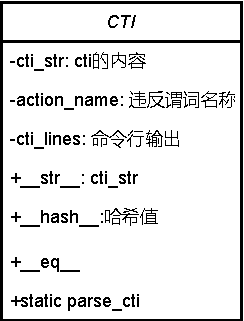
\includegraphics[width=0.3\textwidth]{figures/class_cti.pdf}
    \caption{CTI 类信息}
    \label{fig:class_cti}
\end{figure}
\section{候选不变式生成模块}

生成模块是本项目的关键,它负责生成候选不变式,检验模块是为生成模块服务的。
不同于以往的归纳不变式生成工具,使用随机枚举的方式生成候选不变式,我们引入强化学习来提高我们枚举的效率和成功率。
强化学习是一种通过智能体和环境的交互,智能体通过观察环境的状态,采取行动,获得奖励,来学习如何在环境中获取最大的奖励。
如图\ref{fig:rl}所示,一个强化学习模块可以分为智能体和环境两个部分。

\subsection{强化学习环境实现}

环境接收智能体的行动,做出反应并返回自身的状态和奖励,智能体根据环境的状态和奖励,调整滋生的策略,做出行动的选择。
本文使用\href{https://gymnasium.farama.org/}{gymnasium} \cite{gymnasium} 实现强化学习的环境。
gymnasium是一个开源的强化学习环境,提供了标准的环境接口,方便用户实现自己的强化学习环境,为我们实现环境提供了诸多便利。

自定义一个基于 gymnasium 的环境,最重要的是定义好环境的 \textbf{action\_space} 和 \textbf{observation\_space},以及实现step 函数。

\textbf{action\_space} 和 \textbf{observation\_space} 的数据类型都基于gymnasium的Space类,这其中包括众多类型。
\textbf{action\_space} 代表智能体所能采取的行动的空间,我们这里选择了\textbf{MultiDiscrete},智能体选择的行动为一个等同如输入的 \textbf{predicates} 长的向量。
这个向量每个维度的值都只能是0, 1, 2。在后续,我们会给这个向量 -1,得到一个每个维度上只有-1, 0, 1的向量,这个向量代表了我们的候选不变式。
每个维度上的值代表着对应的谓词是否被选择,-1代表否定,0代表不确定,1代表肯定。
向量与谓词相乘,便可以得到一个谓词表达式,再在前面加上定义好的量词,便可以得到一个候选不变式。

\textbf{observation\_space} 代表智能体所能观察到的环境的空间。
这里选择了\textbf{Dict} 类型。给予智能体参考的信息有:当前的不变式,对于当前不变式的反例或者归纳反例,可以选择的谓词,已经加入归纳不变式的不变式。
\textbf{Dict} 中每个键所对应的值也必须是一个Space类型,对于这四条信息,都选择了\textbf{Text}类型,也就是对应于字符串。

\textbf{step} 函数是环境的核心,它接受智能体的行动,返回环境的观察值,奖励和是否终止。
在我们的环境中,智能体的行动是一个向量,我们需要将这个向量转化为一个候选不变式,然后交给检验模块进行验证。
如果得到了归纳不变式,会给予100的奖励并退出。除此以外的所有情况,因为没有得到归纳不变式,所以都不会推出。
如果得到一个合适的不变式,会给予10的奖励,如果得到了一个错误的不变式,会给予-10的奖励。
如果得到一个不变式,但是不“独立”,会给予2的奖励,但是如果智能体简单地将正确的不变式合取上一个新的谓词,会给予-2的奖励。
与此同时,\textbf{step} 函数还需要返回观察值,这对应于observation\_space中的四条信息的数据结构。
这里复用了反例字段,在得到合适不变式时,返回归纳反例,否则,返回的是智能体提供的不变式的反例。
% 配个图
\begin{table}[!h]
    \label{table:award_punish}
	\centering
	\caption{奖励与惩罚的情况设置}
	\label{tab::situation}
	\renewcommand\arraystretch{1.4}
	\begin{tabular}{p{0.25\textwidth}p{0.15\textwidth}p{0.5\textwidth}}
		\toprule
		\textbf{候选不变式结果}   & \textbf{奖惩值} \\ 
        \midrule
		简单重复已有不变式 & -10 \\
		非不变式      & 0   \\
		被已有不变式覆盖  & 2   \\
		归纳不变式子式   & 10 \\
        \bottomrule
	\end{tabular}
\end{table}

\subsection{强化学习智能体实现}

实现智能体并不困难,gymnasium 的环境接口可以对接诸多的强化学习智能体实现框架。
本文选择了OpenAI \href{https://github.com/openai/baselines}{baselines}\cite{baselines}来实现智能体部分。
baselines 包括多种强化学习算法。
本文尝试了多种算法,包括DQN,PPO,A2C等算法。

\section{非功能模块}

非功能模块包括日志功能,计时功能,报错信息等,这些功能伴随着系统每个行为,为开发人员和用户提供更多信息,方便调试和使用。